\section{Future Upgrades}
\label{sec:FutureUpgrades}

\subsection{High Luminosity LHC}
\label{subsec:HLLHC}
The planned High Luminosity Large Hadron Collider (HL-LHC) is expected to operate starting mid-2029. The primary goals of HL-LHC are to collect large quantities of high-quality data statistics needed to study rare SM processes such as Higgs self-interaction, Higgs couplings to lighter particles, the longitudinal component of vector boson scattering processes, and to extend the direct BSM searches beyond the current reach of LHC. The HL-LHC upgrade aims to increase the center-of-mass energy of proton-proton collisions to $\sqrt{s}=14$ TeV and the instantaneous luminosity up to $\mathcal L = 7.5 \times 10^{34} cm^{-2}s^{-1}$ \cite{HLLHC}. Figure \ref{fig:HLLHC} shows the complete operation of LHC starting in 2011 to the planned decade-long HL-LHC program. 

\begin{figure}[!htb]
    \centering
    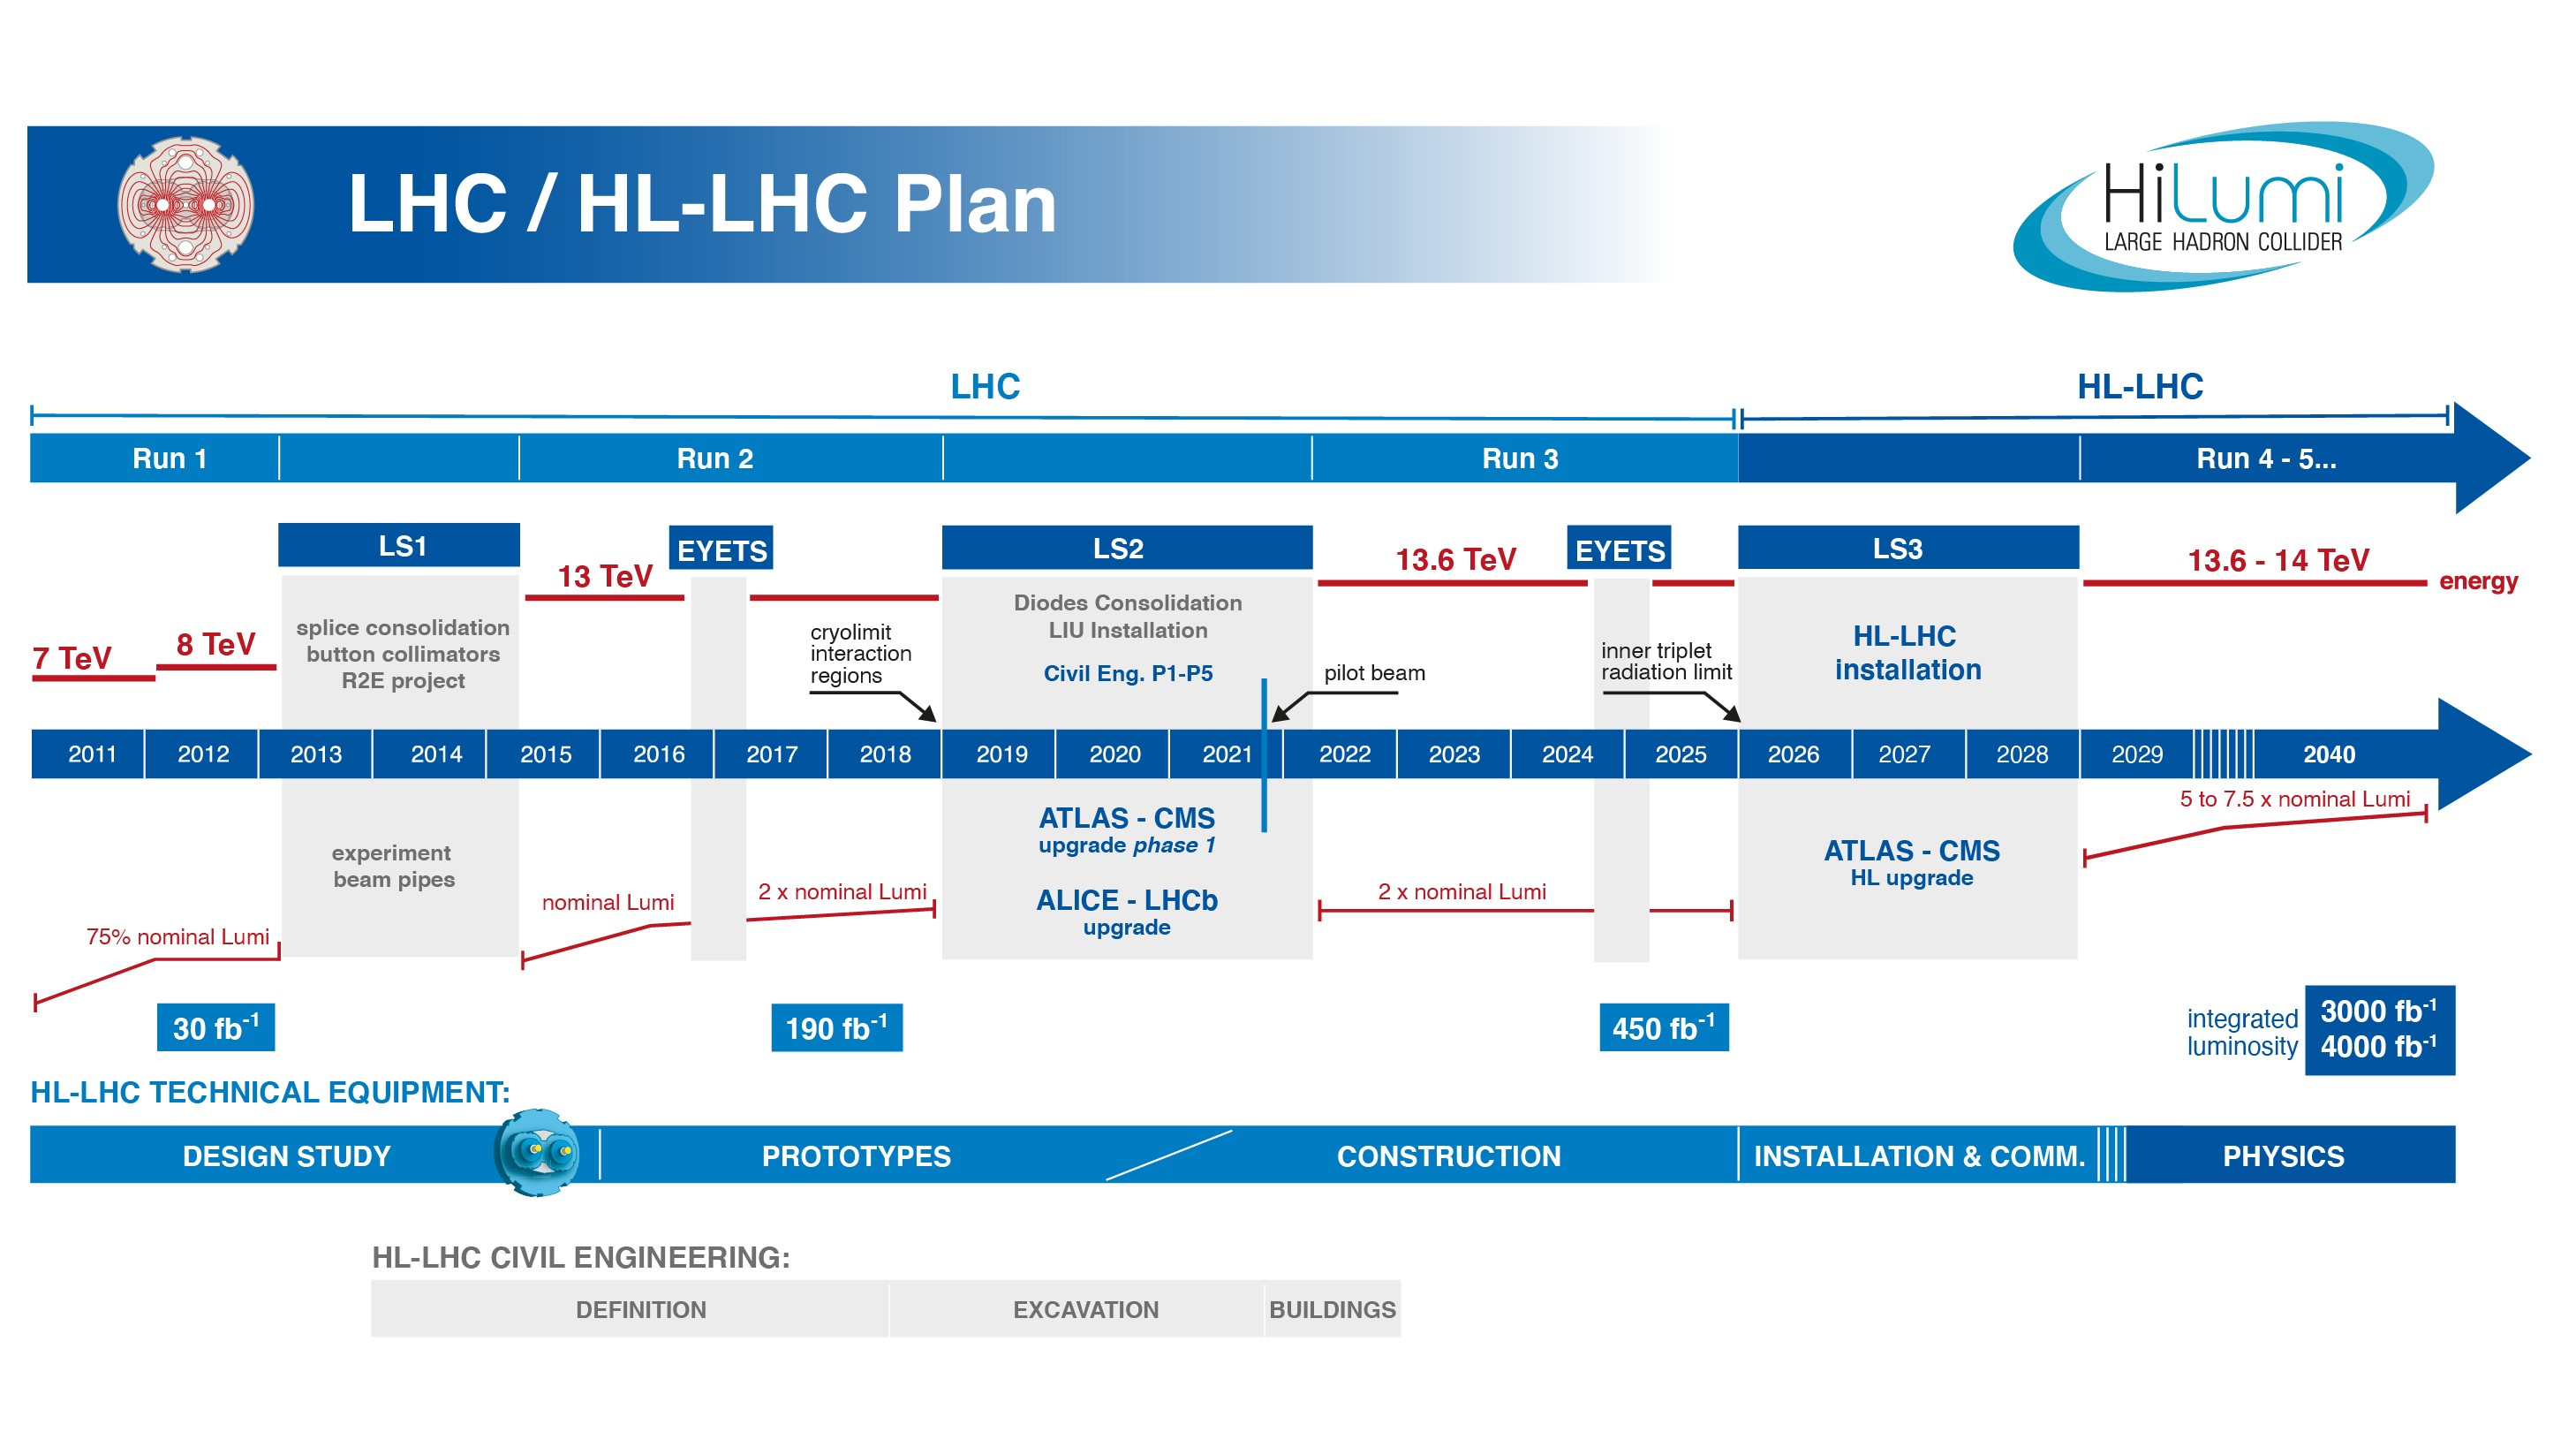
\includegraphics[width=.95\linewidth]{figures/LHC/HLLHCPlan.jpeg}
    \caption{ Timeline of LHC operation starting from 2011 to planned HL-LHC upgrade. Taken from \small{https://hilumilhc.web.cern.ch/content/hl-lhc-project}.\label{fig:HLLHC}}
\end{figure}
\normalsize

\subsection{ATLAS Upgrades}
\label{subsec:ATLASUpgrade}
At HL-LHC, about $200$ interactions per bunch crossing are expected, giving rise to several detector challenges, such as higher detector occupancy, harsher radiation conditions, and higher particle fluxes \cite{HLLHC}. The atlas detector will undergo a Phase-II upgrade to upgrade several sub-systems of ATLAS to meet the challenges of HL-LHC. The main upgrades include upgrading the muon system by adding new chambers in the inner barrel region, upgrading the trigger $\&$ data acquisition system to meet challenges from higher detector occupancy, and upgrading the electronics of several sub-systems. A new High Granularity Timing Detector (HGTD) will also be inserted in the end-cap regions to supplement the tracking system. Most importantly, the current ID will be replaced by all-Silicon Inner Tracking (ITk) detector \cite{HLLHC}.

The ITk consists of Silicon pixel and strip detectors to increase granularity and radiation hardness with less material in the detector. Figure \ref{fig:ITKLayout} schematically shows the ITk layout with $5$ inner layers of pixel detector and four outer layers of strips detector. The tracking for ITk is extended in the forward region up to $|\eta| < 4.0$ region \cite{ITkStripsTDR}. 

\begin{figure}[!htb]
    \centering
    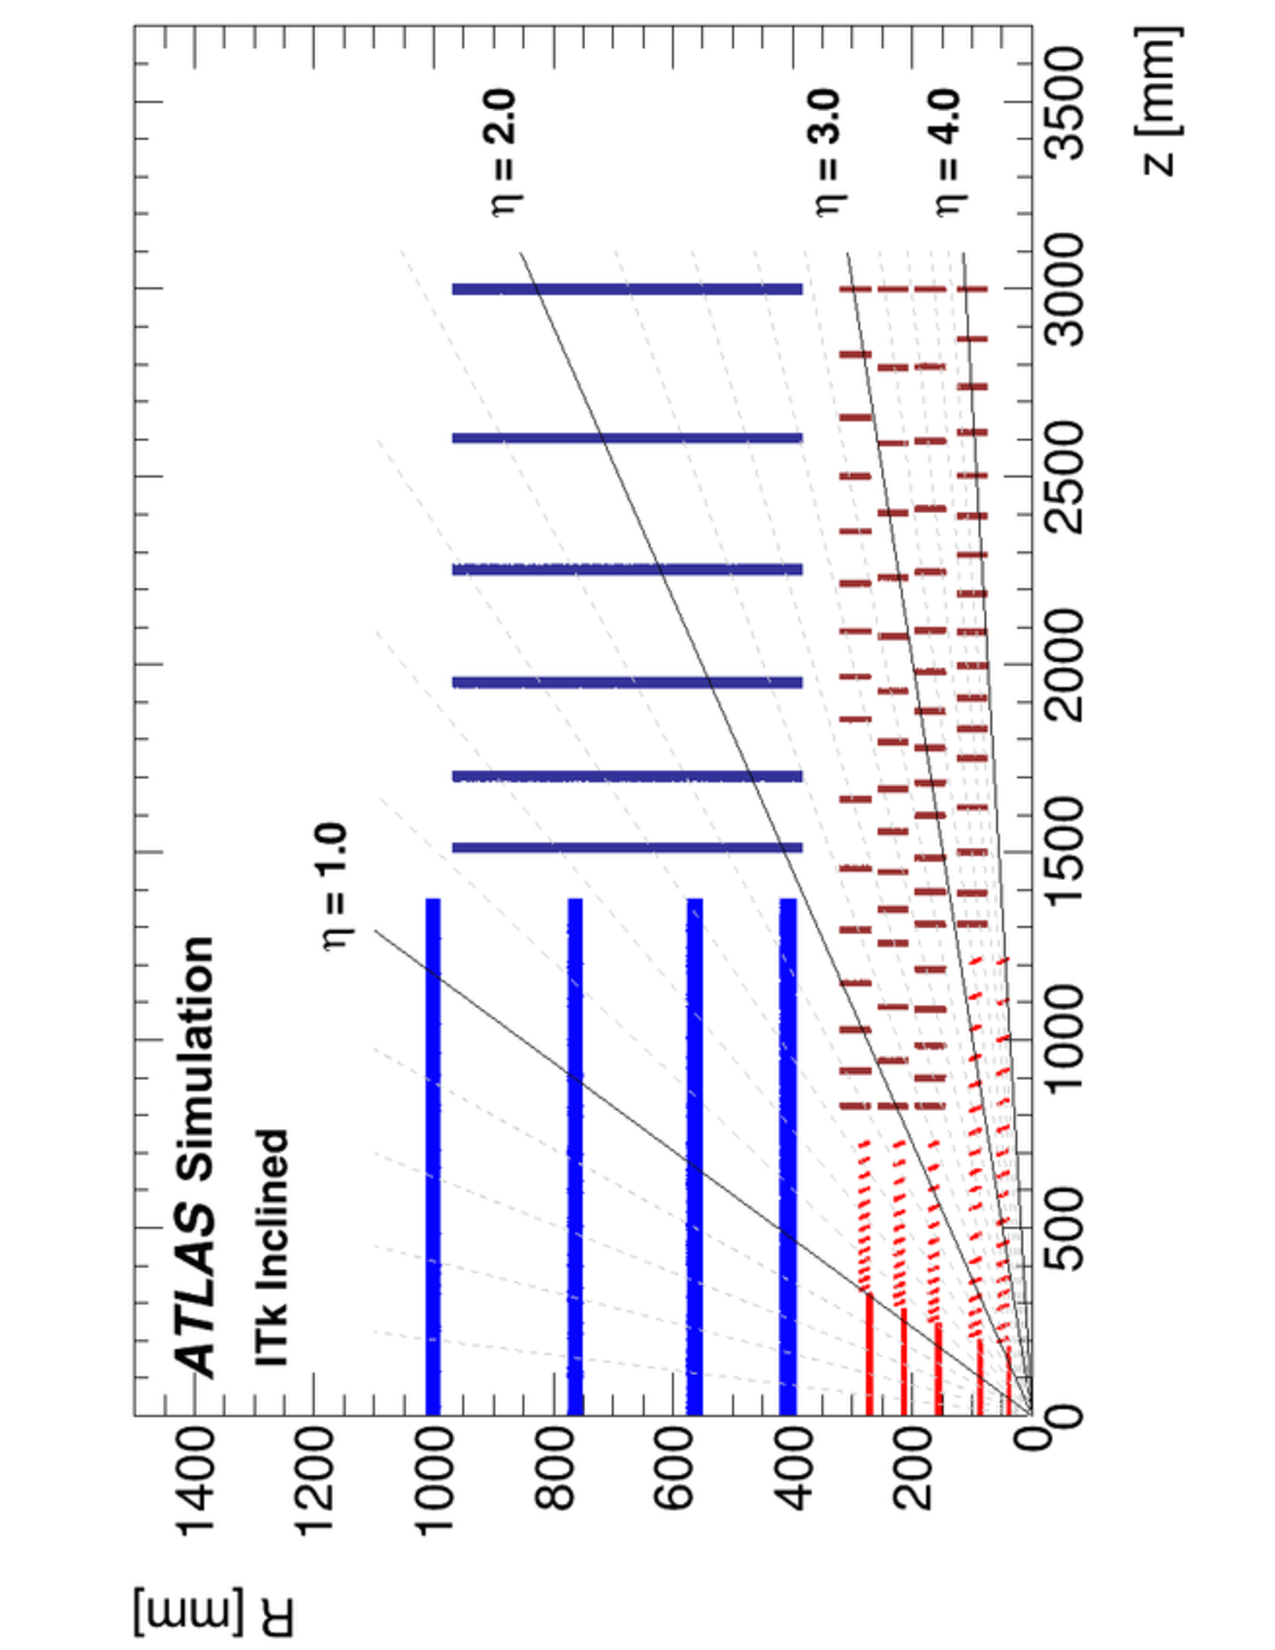
\includegraphics[angle=270,width=.7\linewidth]{figures/LHC/ITKLayout.pdf}
    \caption{ Schematic layout of ITK \cite{ITkPixelTDR}.\label{fig:ITKLayout}}
\end{figure}

More extensive statistics, extended tracking in the forward region, and the timing information from the HGTD in HL-LHC program are highly beneficial to VBS $ZZjj$ measurements with extremely small cross-sections and two jets in the forward regions. 